\section{Data models and formats}

This section gives an overview of the current status and plans for the gamma-ray data model and formats. As mentioned before, this effort was only started recently and none of the formats should be considered stable. The next two sections will describe the effort to define an event data model and format (DL3) and higher-level formats for sky-maps, spectra, and lightcurves (DL4), i.e. a content split as already illustrated in Figure~\ref{fig:purpose}.
In the data specification document we have created a ``general'' section where common quantities are defined, such as precise definitions of time scales as well as coordinate systems. 
%
There are some general topics still under discussion, e.g. there is no consensus on how specific or flexible the format specifications should be. E.g. some people prefer to be very specific (data must be stored in FITS files, data types and units fixed), others would prefer to be flexible (only define header keywords and column names, but data can be stored in other file formats as well, e.g. text-based formats like ECSV).

\subsection{Data level 3 specifications}

The interface between low-level (calibration, shower reconstruction, gamma-hadron separation) and high-level (science tools) analysis for gamma-ray data is usually represented by an event list, where at a minimum the \texttt{EVENT\_ID}, \texttt{TIME}, as well as the reconstructed \texttt{ENERGY} and sky position (\texttt{RA}, \texttt{DEC}) is given for every event. In addition, instrument response functions (IRFs) as well as auxiliary technical information such as telescope configuration options, good time intervals (GTIs), live-time, and pointing information (collectively called \texttt{TECH} in the CTA context) are needed by the science tools to compute exposures, effective resolutions (PSF and EDISP), and ultimately fluxes to compare the data with sky models. This DL3 data, illustrated in Figure~\ref{fig:iact-dl3}, is similar for all gamma-ray telescopes (and other event-recording instruments like e.g. neutrino telescopes). One major difference that affects data formats and analysis tools is whether the gamma-ray telescope was operated in a pointed observation mode (like IACTs most of the time) or in a slewing mode (like HAWC or Fermi-LAT most of the time).

\begin{figure}[tb]
\centerline{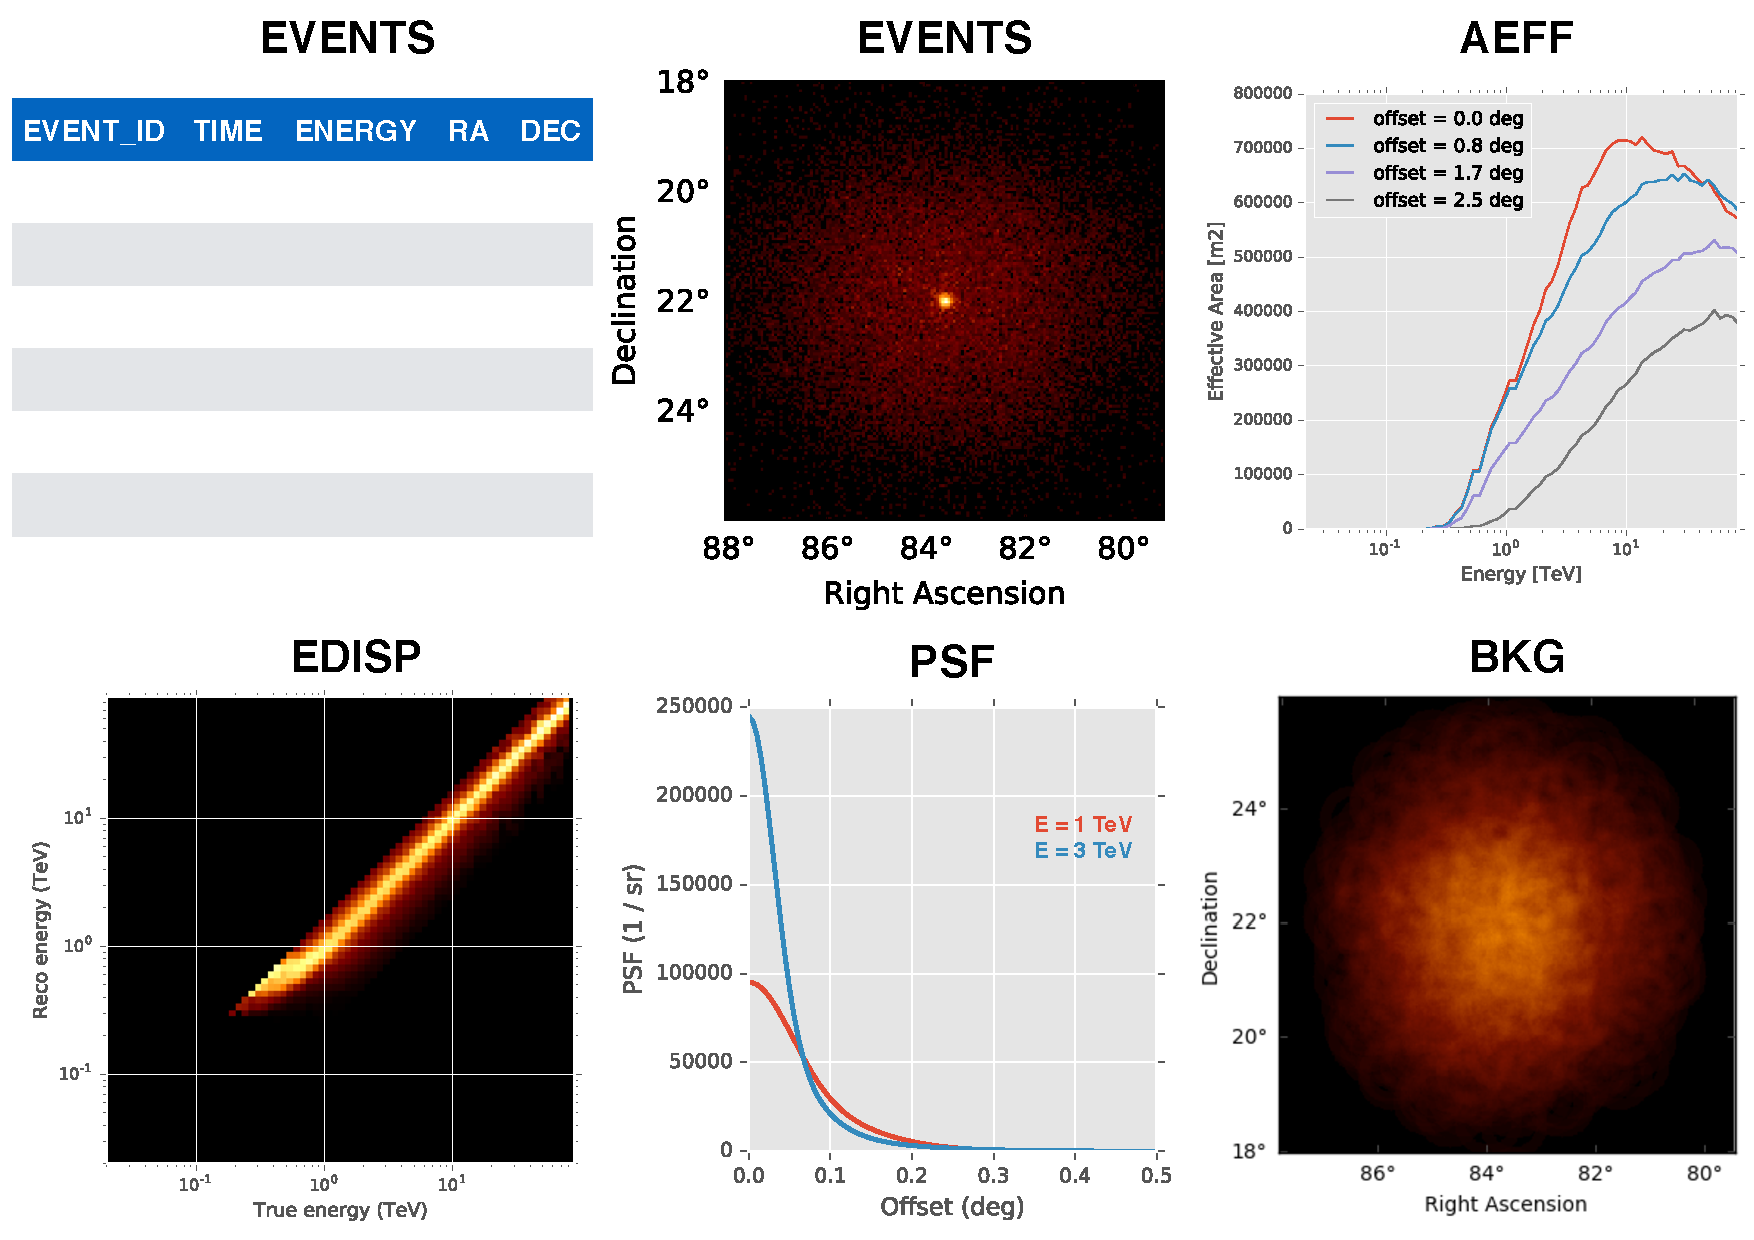
\includegraphics[width=0.8\textwidth]{figures/iact-dl3}}
\caption{
Illustration of major components of IACT DL3 data (using a H.E.S.S. 1 Crab nebula observation). The \texttt{EVENTS} are stored as a table with the most relevant parameters shown. To derive spectra and morphology measurements of astrophysical sources, instrument response functions (IRFs) are used: effective area (\texttt{AEFF}), energy dispersion (\texttt{EDISP}), and point spread function (\texttt{PSF}). Sometimes background (\texttt{BKG}) models are also created and released as part of DL3 data (as an additional IRF component), and other times they are derived at the science tools level. Note that this picture is not complete, see the ``IACT DL3'' section.
}
\label{fig:iact-dl3}
\end{figure}

The current specification contains a very preliminary proposal of a data model and formats for IACT DL3 data that is based on ``observations'' (with an \texttt{OBS\_ID}) and assumed stable IRFs during the observation. This proposal was inspired by existing formats used by H.E.S.S. and partly also VERITAS and MAGIC, that are mostly supported by the existing science tool prototypes (Gammapy and ctools). 
% Remove this sentence ... mainly to save space (6-page limit)
% To help the \gadf effort and science tool prototyping, H.E.S.S. is planning to release a small test dataset in the current format consisting of roughly 50 hours of H.E.S.S. 1 observations on a few sources in fall 2016.
A dedicated two-day face-to-face meeting on IACT DL3 data was held in April 2016 in Meudon, France, with 16 participants from all major existing IACTs and CTA.\footnote{\ogrameudon} The use cases and status of efforts to export and archive their data in FITS was presented, as well as the ongoing prototyping in science tools. Many important points were discussed:
%
\begin{itemize}
\item{}What is an observation? Good time interval? Response time interval?
\item{}How to link \texttt{EVENT} and \texttt{IRF}? (naming conventions, header references, index tables)
\item{}Pointing and live time information
\item{}Exact definition of field of view (FoV) coordinates
\item{}\texttt{IRF} axis specification, validity ranges, errors
\item{}How to support multiple \texttt{EVENT} classes and types?
\end{itemize}
%
A major result of the face-to-face workshop was to agree to focus on IRF formats that use the multi-array convention and FITS BINTABLE to store the IRF data and axis information, where previously a second format was being developed and prototyped for CTA \citep{2015arXiv150807437W}. The prototyping of IACT DL3 is continuing in the different IACT collaborations and in Gammapy/ctools, with communications online via Github, monthly joint tele-conferences, and a planned face-to-face follow-up meeting in fall 2016. So far the focus is set on pointed gamma-ray observations. Contributions and involvement from people working on slewing telescopes (e.g. Fermi-LAT or HAWC and also IACTs) or non-gamma-ray telescopes with similar data (e.g. neutrino telescopes) are welcome. The largest stakeholder for the IACT DL3 work is CTA.

\subsection{Data level 4 \& 5 specifications}

Another topic in the \texttt{gamma-astro-data-formats} specifications is the development of formats to store high-level data products such as sky-maps, spectra, and lightcurves (data level 4) or source catalogs (data level 5).  Here we list DL4 and DL5 format specifications that are currently included in \gadf or under consideration:

\begin{itemize}
\item{} For 2-dimensional images, the existing FITS and world coordinate system (WCS) standard provides a solution that works for gamma-ray sky-maps as well. If something gamma-ray specific were to be added, it would likely be specifications on how to store parameters of interest for analysis or provenance in the header.
\item{} For 3-dimensional cubes, where the third dimension is \texttt{ENERGY}, commonly 3-dimensional \texttt{FITS IMAGE} extensions are used. However, due to either the complexity or missing features in the FITS WCS model, the energy axis information is not represented in the FITS header, but in a separate \texttt{BINTABLE HDU} called \texttt{ENERGY} (if the cube represents quantities at given energies, like exposure or flux), or \texttt{EBOUNDS} ("energy bounds", if the cube represents integral quantities like e.g. counts).
A specification at \gadf can document the exact semantics for storing the energy axis and how interpolation and integration should be performed by science tools (e.g. for exposure or diffuse model flux cubes).
\item{} For all-sky maps and cubes, HEALPix\cite{2005ApJ...622..759G} is commonly used in gamma-ray astronomy (e.g. by Fermi-LAT). While 2-dimensional HEALPix images are standardized, extensions have been developed to represent cubes, as well as to store sparse data or images that don't cover the whole sky \footnote{\pointlikedata}. These gamma-ray specific extensions are not standardized, and a specification at \gadf would be welcome.
\item{} The common method for 1-dimensional spectral analysis in X-ray astronomy \citep{Davis:2001}, as well as the corresponding file formats (e.g. \texttt{ARF} for effective area, \texttt{RMF} for energy dispersion) are also used in VHE gamma-ray astronomy. In the current specification we have added a section referencing the relevant OGIP documents and explained how the formats are commonly used in gamma-ray astronomy (e.g. using a ``reconstructed energy'' axis instead of the ``pulse height channels'' axis used in X-ray astronomy).
\item{} For 1-dimensional spectra, a format to store flux points and upper limits, as well as full likelihood profiles, is available at \gadf (see Figure~\ref{fig:dl4-examples} left panel). It was first developed in Fermipy and applied to Fermi-LAT analyses, and is now being adopted for IACT spectra.
\item{} No format specification for light curves (see Figure~\ref{fig:dl4-examples} right panel for an illustration) is available yet. Previously a format has been proposed in \cite{2010AnA...524A..48T} and a pull request with discussions for a lightcurve specification at \gadf is ongoing.
\item{} No format specifications have been proposed for catalogs (data level 5, DL5) yet. So far each catalog (Fermi-LAT, upcoming H.E.S.S. and HAWC) is unique (but all similar) and some science tools have per-catalog code to produce corresponding sky models.
\end{itemize}

\begin{figure}[tb]
\centerline{\includegraphics[width=0.8\textwidth]{figures/dl4-examples}}
\caption{
Gamma-ray ``data level 4'' examples. \emph{Left:} spectral energy distribution (SED) likelihood profiles (green), with flux points, upper limits and best-fit model shown. \emph{Right:} Lightcurve of 3FGL~J0349.9-2102 from the third Fermi-LAT catalog.
}
\label{fig:dl4-examples}
\end{figure}
